% First Graph (Top image)
\begin{minipage}{0.48\textwidth}
    \centering
    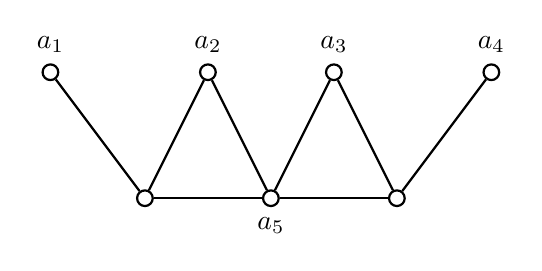
\begin{tikzpicture}[scale=0.8, thick]
        % Define nodes
        \node[circle, draw, inner sep=2pt, label=above:{$a_1$}] (a1) at (0, 2) {};
        \node[circle, draw, inner sep=2pt]                      (u1) at (1.5, 0) {};
        \node[circle, draw, inner sep=2pt, label=above:{$a_2$}] (a2) at (2.5, 2) {};
        \node[circle, draw, inner sep=2pt, label=below:{$a_5$}] (a5) at (3.5, 0) {};
        \node[circle, draw, inner sep=2pt, label=above:{$a_3$}] (a3) at (4.5, 2) {};
        \node[circle, draw, inner sep=2pt]                      (u2) at (5.5, 0) {};
        \node[circle, draw, inner sep=2pt, label=above:{$a_4$}] (a4) at (7, 2) {};

        % Draw edges
        \draw (a1) -- (u1);
        \draw (u1) -- (a2);
        \draw (u1) -- (a5);
        \draw (a2) -- (a5);
        \draw (a5) -- (a3);
        \draw (a5) -- (u2);
        \draw (a3) -- (u2);
        \draw (u2) -- (a4);
    \end{tikzpicture}
\end{minipage}\hfill
% Second Graph (Bottom image)
\begin{minipage}{0.48\textwidth}
    \centering
    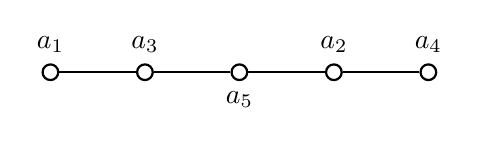
\begin{tikzpicture}[scale=0.8, thick]
        % Define nodes
        \node[circle, draw, inner sep=2pt, label=above:{$a_1$}] (a1) at (0, 0) {};
        \node[circle, draw, inner sep=2pt, label=above:{$a_3$}] (a3) at (1.5, 0) {};
        \node[circle, draw, inner sep=2pt, label=below:{$a_5$}] (a5) at (3, 0) {};
        \node[circle, draw, inner sep=2pt, label=above:{$a_2$}] (a2) at (4.5, 0) {};
        \node[circle, draw, inner sep=2pt, label=above:{$a_4$}] (a4) at (6, 0) {};

        % Draw edges
        \draw (a1) -- (a3);
        \draw (a3) -- (a5);
        \draw (a5) -- (a2);
        \draw (a2) -- (a4);
    \end{tikzpicture}
\end{minipage}
